% !TEX root = thesis-main.tex

\chapter{Data Augmentation for Rare Words}
\label{chapter:research-02}

\section{Introduction and research questions}

In the previous chapter, we observed the impact of context on learning word representations, in particular, modeling polysemy which is a challenging phenomenon in language. 
In the following chapters of this thesis, we investigate other challenges in learning word meaning. 
One medium to evaluate language understanding is machine translation. 
A machine translation system needs to understand the meaning in the source language and transfer it into the target language. 

The quality of a neural machine translation system depends substantially on the availability of sizable parallel corpora.
To train NMT models with reliable parameter estimations, these networks require numerous instances of sentence translation pairs with words occurring in diverse contexts, which is typically not available for low-resource language pairs.
As a result, NMT falls short of producing good-quality translations for these language pairs \citep{zoph-EtAl:2016:EMNLP2016,koehn2017six,gu-etal-2018-meta,ngo-etal-2019-overcoming}.
The solution is to either revise the learning models \citep{ostling2017neural}, or to provide more training data by manual annotation \citep{Melamed98manualannotation} or to perform automatic data augmentation \citep{sennrich-haddow-birch:2016:P16-11,wang-etal-2018-switchout}. 
Since manual annotation of data is time-consuming, data augmentation for low-resource language pairs is a more viable approach.

In computer vision, data augmentation techniques are widely used to increase robustness and improve the learning of objects with a limited number of training examples. 
In image processing, the training data is augmented  
by, for instance, horizontally flipping, random cropping, tilting, and altering the RGB channels of the original images \citep{NIPS2012_4824,DBLP:conf/bmvc/ChatfieldSVZ14}. Since the content of the new image is still the same, the label of the original image is preserved (see Figure~\ref{augfig}: top).
While data augmentation has become a standard technique to train deep networks for image processing, it is not common practice for training networks for NLP applications such as machine translation.

\begin{figure}
\centering
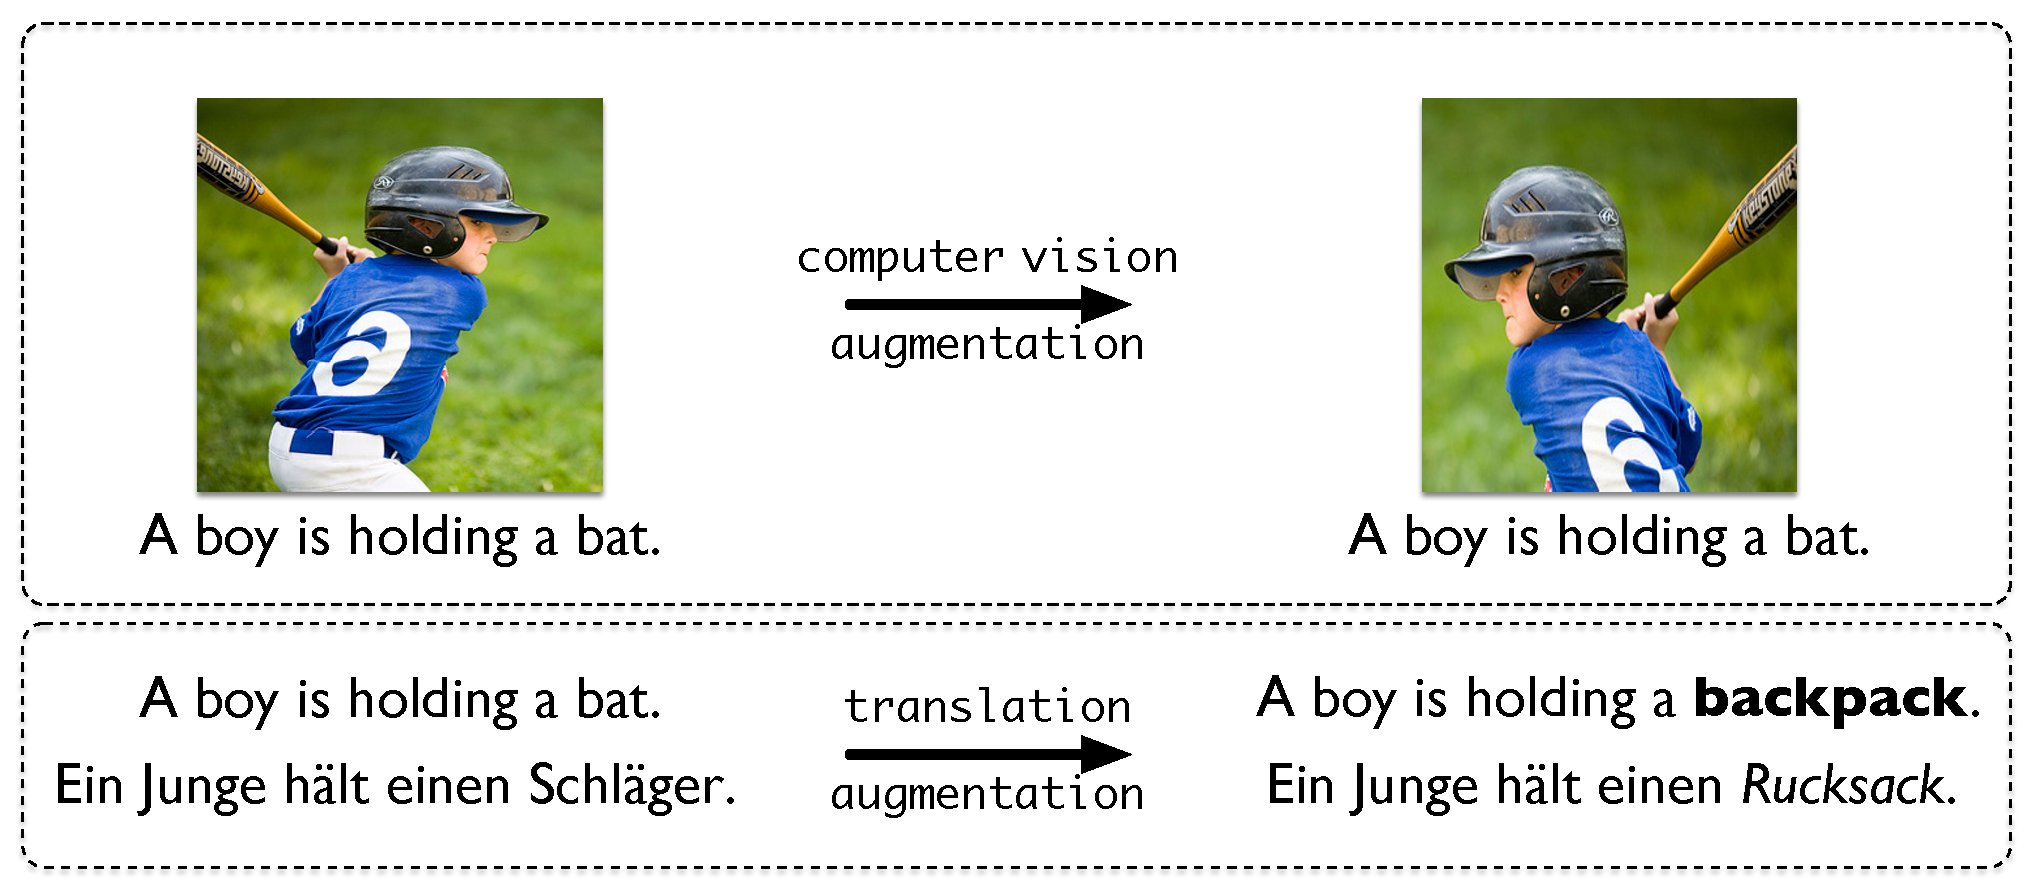
\includegraphics[width=0.75\linewidth]{04-research-02/figs/augomni2.pdf}
\caption{Top: %A data augmentation technique to alter an image where the description remains the same. 
flip and crop, two label-preserving data augmentation techniques in computer vision.
Bottom: Altering one sentence in a parallel corpus requires changing its translation.}
\label{augfig}
\end{figure}


In this chapter, we address the challenge of translation of low-resource language pairs where the primary obstacle is the lack of sufficient training data.
Motivated by the success of data augmentation in computer vision, we investigate in this chapter whether NMT can benefit from data augmentation as well.
Concretely, we ask:


\paragraph{Research Question 2:} \acl{rq:tdabt} 

\medskip

 \noindent Research has shown that there is a strong correlation between the size of the training data and the quality of neural models \citep{Halevy:2009:UED:1525642.1525689}.
To investigate this relation in machine translation, we compare how the translation and generation of a word changes by adding diverse contexts to the training data.  
In this chapter, we focus on low-resource language pairs, simulating a low-resource setting as done in the literature \citep{Marton:2009:ISM:1699510.1699560,duong-EtAl:2015:EMNLP},  to examine the effects of the lack of data on translation quality.
In particular, we look into the translation and generation of rare words, thus asking: 
 
\begin{enumerate}[label=\textbf{RQ2.\arabic* },wide = 0pt, leftmargin=2em]
\setlength\itemsep{1em}
\item \acl{rq:tda1}

\medskip

\noindent The impact of training data scarcity on translation quality is especially noticeable for rare words \citep{sennrich-haddow-birch:2016:P16-12}. 
%Our quantitive analysis starts with examining rare words in a low-resource setting. 
We demonstrate that parameter estimation of rare words is challenging in NMT, and it is further exacerbated in a low-resource setting.
%Concretely, we measure the quality of translation and generation of these words.
We investigate the effects of additional context, generated automatically, on both \textit{translating} and \textit{generating} rare words. 
We achieve this by proposing a simple yet effective approach that augments the training data by altering existing sentences in the parallel corpus, similar in spirit to the data augmentation approaches in computer vision (see Figure~\ref{augfig}).
First, we propose a weaker notion of label preservation that allows altering both source and target sentences at the same time as long as they remain translations of each other. 
%We obtain substantial improvements for translating English$\rightarrow$German and German$\rightarrow$English.

Next, we examine augmentation during \textit{test time} by exploring a stronger notion of label preservation, and we ask: 

\item \acl{rq:tda2}

\medskip

\noindent For the augmentation process in this scenario to be possible, any change to a sentence in one language must preserve the meaning of the sentence.  
It is essential because we aim for not altering reference translations during evaluation. 
We hypothesize that it should be useful to alter the source sentence containing a rare or out-of-vocabulary word by paraphrasing it with a more common word.
In addition, we also investigate the performance of different paraphrasing resources.

\end{enumerate}


\paragraph{Organization.} This chapter is organized as follows: 
After reviewing the previous work (Section~\ref{tda:background}), we present our main data augmentation model in Section~\ref{tda:model}. 
In Section~\ref{tda:exp}, we introduce the general experimental setup, followed by a detailed description of the results of the translation experiments in Section~\ref{tda:results}. 
We analyze the effectiveness of the model further in Section~\ref{tda:analysis}.
Next, we discuss augmentation at inference and propose a meaning-preserving method in Section~\ref{tda:semantic}. 
Finally, we conclude in Section~\ref{tda:conc} with an outlook of future work.


\section{Previous work} \label{tda:background}

Relevant previous work for the work described in this chapter involves two research topics: 
First, we briefly review the literature on image data augmentation.
Second, we discuss researches studying challenges in translation of low-resource language pairs.
%We also briefly present previous work on neural language modeling. 

\subsection{Data augmentation in computer vision}

Neural models learn best when massive data is available \citep{Halevy:2009:UED:1525642.1525689}.
As a result, data augmentation has become one of the staple preprocessing steps in image classification \citep{NIPS2012_4824,huang2018gpipe, cubuk2019autoaugment}, image generation \citep{kynkaanniemi2019improved,karras2019style}, and object detection \citep{singh2018sniper,liu2016ssd}.
Data augmentation approaches address the overfitting problem in neural models from the perspective of the training data. 
Extensive research in computer vision has been done over the years on different techniques of data manipulation. 
There are various techniques to manipulate image data. For instance:

\begin{itemize}
 \item \textbf{Geometric transformations:} These changes are simple alterations that are applied to the images in the training data---for instance, flipping, rotation, and cropping. 
    
    \item \textbf{Mixing images:} These transformations are done by combining multiple images either from the same class or sampled from the entire training data---for instance, averaging pixel values of multiple images or randomly cropping and patching images. \citet{inoue2018data} show that by overlaying images and augmenting data, they achieve significant improvements in classification accuracy on CIFAR-100 data set.
\end{itemize}

Note that the augmentation techniques in computer vision have hardly any concerns about whether the image still \textit{remains} an equivalent image after the alteration. 
That is not the case for augmentation of sentences, where any alteration should be mindful of generating semantically and syntactically correct sentences. 

\begin{comment}
\begin{table}
\centering
\small
\begin{tabularx}{\linewidth}{lll}
 \toprule
\textbf{Technique} & \textbf{Augmentation strategy} &   \\ \midrule
\multirow{5}{*}{Data warping}  &  Geometric transformations & \\
& Kernel filters & \\
& Color space transformation & \\
& Random erasing & \\
& Mixing images & \\ \midrule
\multirow{3}{*}{Deep learning approaches} & Adversarial training & \\
& Neural style transfer & \\
& GAN data augmentation & \\
\bottomrule
\end{tabularx}
\caption{blah}
\label{backgroundcomputervision}
\end{table}
\end{comment}


\subsection{Low-Resource translation}

Parallel data, which is the primary source of learning for machine translation models, is constructed manually and is not available in abundance for every language pair (see Section~\ref{databg}). 
Neural translation models especially suffer from the lack of sufficient parallel data for training. 
\citet{koehn2017six} experiment with different corpora sizes and show that their NMT system only outperforms their phrase-based machine translation system when more than 100 million words of parallel data are available. 
However, \citet{sennrich-zhang-2019-revisiting} show that NMT models are highly sensitive to hyperparameters such as BPE vocabulary size. They observe strong improvements by adapting system parameters to low-resource settings.  

Additionally, in a low-resource setting, the problem of translating rare words is more pronounced. 
Both \citet{sutskever2014sequence} and \citet{DBLP:journals/corr/BahdanauCB14} observe that NMT models tend to translate sentences with many rare words more poorly than sentences containing mostly frequent words.
Several recent approaches have targeted the low-resource obstacle in machine translation in different ways. 
Based on their approach and viewpoint on addressing this problem, current research can be categorized into four main groups:

\paragraph{Leveraging monolingual data} 
We discussed several approaches to leverage monolingual data in translation in Section~\ref{bgbtref}.
These approaches address the problem by leveraging data resources other than the limited parallel corpora. 
\citet{sennrich-haddow-birch:2016:P16-11} propose a method to back-translate sentences from monolingual data and augment the bitext with the resulting pseudo-parallel corpora.  %This approach results in significant improvements in many language pairs.
While this approach is successful in improving the translation quality, it is not effective in very low-resource settings where the back-translation model cannot be trained to a sufficient level of quality \citep{abdulmumin2020using}.
This approach is further discussed in Chapter~\ref{chapter:research-03}.
\citet{currey2017copied} create a parallel corpus from monolingual data in the target language by copying it so that each source sentence is identical to its corresponding target sentence. With this simple technique, they observe improvements on relatively low-resource language pairs such as English$\leftrightarrow$Turkish and English$\leftrightarrow$Romanian.


\paragraph{Re-designing the model} 
These approaches target the model itself and propose changes to the standard neural translation models \citep{costa-jussa-fonollosa-2016-character,sennrich-haddow-birch:2016:P16-12}.
\citet{ostling2017neural} propose to learn sentence reordering during translation of low-resource language pairs by introducing more local dependencies.
They use word alignments to provide supervision to the reordering model.
\citet{lee-etal-2017-fully} introduce a fully character-level translation model that maps a character sequence in a source language to a character sequence in a target language. 
They observed significant improvements in the translation of morphologically rich languages where the word-level NMT models fail to translate rare and out-of-vocabulary words.
Previous approaches which propose different segmentations of the input sequence are effective; however, they present a different set of challenges:
With longer sequences, the model requires information to be retained over longer temporal spans. 
Moreover, since the meaning of a word is not a compositional function of its characters, the model must learn to memorize many character sequences as higher-level linguistic abstractions. \citep{cherry-etal-2018-revisiting}.

\paragraph{Cross-lingual transfer learning}
These strategies use models trained on high-resource language pairs to transfer various parameters and components to the low-resource language pair. 
\citet{zoph-EtAl:2016:EMNLP2016} propose to train a high-resource language pair first and then transfer some of the learned parameters to the low-resource pair to initialize and constrain training. 
\citet{gu2018universal} show that sharing lexical and sentence-level representations across multiple source languages aid in the translation of low-resource languages. They also use monolingual embeddings along with seed parallel data from all languages to build a universal representation.
Cross-lingual approaches are particularly valuable for multilingual translation learning, where a single NMT model learns to translate between multiple languages \citep{firat-etal-2016-multi,johnson-etal-2017-googles,blackwood-etal-2018-multilingual,aharoni-etal-2019-massively}.
While these approaches are very impressive in translating between language pairs not seen during training, this paradigm cannot outperform the individual models trained on bilingual corpus in many cases \citep{johnson-etal-2017-googles}.


\paragraph{Unsupervised learning} 
These studies focus on zero-resource learning, where there are no parallel corpora available for a language pair \citep{yang-etal-2018-unsupervised,artetxe-etal-2018-unsupervised,artetxe2018iclr,artetxe-etal-2019-effective}.
\citet{lample2018unsupervised} propose a model that takes sentences from monolingual data in two different languages and maps them into the same latent space.
The model learns to translate without using any parallel data by reconstructing both languages from the shared feature space. 
\citet{lample-etal-2018-phrase} address the challenge of only having access to monolingual corpora in each language. 
They use a smoothed n-gram language model (phrase-based model) as a data-driven prior to denoising sentences and automatically generate the parallel data by iterative back-translation (neural model).
%, they achieve impressive results. 
These approaches are effective; however, the pseudo sentences used for training are usually of low quality as translation mistakes accumulate during training. 
Additionally, while they perform well between languages that are from the same branch, they perform poorly between distant languages \citep{sun-etal-2020-knowledge}.

%\subsection{Recurrent neural language model} TODO: move to BG chapter

\section{Data augmentation for rare words} \label{tda:model}

In this section, we propose a novel approach for data augmentation of parallel corpora. Specifically, we use a Bidirectional RNN model trained on monolingual data to introduce completely new contexts for rare words in the bitext. In our approach we use sentences from the training data as starting points and use the probability distribution of the output layer of an RNN to insert words into new contexts: 
Given %a pair of 
a source and target sentence pair $(S,T)$, we want to alter it in a way that we obtain new contexts for these words while diversifying as much as possible the training examples.
A number of ways to do this can be envisaged, as for example paraphrasing (parts of) $S$ or $T$, or altering both and preserve the semantic equivalence between $S$ and $T$.
We explore both approaches in this chapter.

We choose to focus on a subset of the vocabulary that we know to be poorly modeled by our baseline NMT system, namely words that occur rarely in the parallel corpus.
Thus, the goal of our data augmentation technique is to provide novel contexts for rare words.
To achieve this we search for contexts where a common word can be replaced by a rare word and consequently replace its corresponding word in the other language by that rare word's translation:
\vspace{1mm}

\begin{center}\small
\setlength{\tabcolsep}{15pt}
\begin{tabular}{ll}
\textbf{original pair} & \textbf{augmented pair} \\\hline
$S: s_1, \ldots , s_i, \ldots, s_n$ & $S': s_1, \ldots , s_i', \ldots , s_n$ \\
$T: t_1, \ldots , t_j, \ldots , t_m$ & $T': t_1, \ldots , t_j', \ldots , t_m$ \\ %\textit{trans}(s_i')
\end{tabular}
\end{center}

\vspace{1mm}

\noindent%
where $t_j$ is a translation of $s_i$ and word-aligned to $s_i$, and $t_j'$ is the translation of $s_i'$.
Plausible substitutions are those that result in a fluent and grammatical sentence but do not necessarily maintain its semantic content.
As an example, the rare word \textit{motorbike} can be substituted in different contexts:

\smallskip

\begin{center}\small
\begin{tabular}{l | l}
Sentence [original \textbackslash \textbf{substituted}] &  \begin{tabular}[x]{@{}c@{}}Plausible\end{tabular}  \\
\hline
	My sister drives a  [car \textbackslash \textbf{motorbike}]  & yes \\
	My uncle sold his [house \textbackslash \textbf{motorbike}] & yes \\
	Alice waters the [plant \textbackslash  \textbf{motorbike}]  & no (semantics) \\
	John bought two [shirts \textbackslash\textbf{motorbike}] & no (syntax) \\
\end{tabular}
\end{center}

\smallskip

\noindent%
%where the third and fourth rows illustrate a semantically and a syntactically wrong context respectively.
%with highlighted [original / \textbf{substituted}] words. 
%Clearly, blindly substituting words can result in semantically or syntactically wrong sentences. %as shown in this table.  (third and fourth examples).
Implausible substitutions need to be ruled out during data augmentation.
To this end, rather than relying on linguistic resources %, like parsers or ontologies, 
which are not available for many languages, %we rule out inappropriate substitutions by using 
we rely on LSTM language models (LM) trained on large amounts of monolingual data in both forward and backward directions.

Our data augmentation method involves the following steps:
%
\paragraph{Targeted words selection:}
Following common practice, our NMT system limits its vocabulary $V$ to the $v$ most common words observed in the training corpus.
We select the words in $V$ that have fewer than $R$ occurrences and use this as our targeted rare word list $V_R$.
\paragraph{Rare word substitution:}
If the LM suggests a rare substitution in a particular context, we replace that word and add the new sentence to the training data.
Formally, given a sentence pair $(S,T)$ and a position $i$ in $S$, we compute the probability distribution over $V$ by the forward and backward LMs and select rare word substitutions $\mathcal{C}$ as follows:
\begin{align}
\overrightarrow{\mathcal{C}} & = \{ s'_i \in V_{R} : \topk  P_{\textrm{\textit{ForwardLM}}_S}(s'_i \given s_{1}^{i-1}) \} \\
\overleftarrow{\mathcal{C}} & = \{ s'_i \in V_{R} : \topk P_{\textrm{\textit{BackwardLM}}_S}(s'_i \given s_{n}^{i+1}) \} \\
\mathcal{C} \ & = \{s'_i \given s'_i \in \overrightarrow{\mathcal{C}} \land s'_i \in \overleftarrow{\mathcal{C}} \} 
\end{align}
where $s_{i}^{j}$ are context words from position $i$ to $j$ and $\topk$ returns the $K$ words with highest conditional probability according to the context. 
The selected substitutions $s'_i$, are used to replace the original word and generate a new sentence.
%
%\footnote{We accept as plausible substitutions the top $k$ words of the vocabulary ranked by the multiplication of forward and backward RNN LM probabilities.}

\paragraph{Translation selection:}
Using automatic word alignments\footnote{We use fast-align \citep{dyer-chahuneau-smith:2013:NAACL-HLT} to extract word alignments and a bilingual lexicon with lexical translation probabilities from the low-resource bitext.} trained over the bitext, we replace the translation of word $s_i$ in $T$ by the translation of its substitution $s_i'$. 
Following a common practice in statistical MT \citep{koehn-etal-2007-moses}, the optimal translation $t'_j$ is chosen by multiplying direct and inverse lexical translation probabilities with the LM probabilities of the translation in context: % the other language (?)}.
\begin{equation}
t'_j =  \mathop{\argmax}_{t \in \textit{trans}(s_i')} P(s'_i \given t) P(t \given s'_i) P_{\textrm{\textit{ForwardLM}}_T}(t \given t_{1}^{j-1}) P_{\textrm{\textit{BackwardLM}}_T}(t \given t_{n}^{j+1})
\end{equation}
%
If no translation candidate is found because the word is unaligned or because
%In case there is no substitution candidate due to no alignment, or 
the language model probability is less than a certain threshold, the augmented sentence is discarded.
This reduces the risk of generating sentence pairs that are semantically or syntactically incorrect.

\medskip

We use the described steps of targeting and substituting words in source and target sentences to augment the training data:

\paragraph{Sampling:}
We loop over the original parallel corpus multiple times, sampling substitution positions $i$ in each sentence and making sure that each rare word gets augmented at most $N$ times so that a large number of rare words can be affected.
We stop when no new sentences are generated in one pass over the training data.

\paragraph{Augmentation:}
Assuming the original parallel data is $\mathcal{D}$, our data augmentation process can be represented by the following mapping:
\begin{equation}
\phi:  \mathcal{D} \mapsto \mathcal{A}
\end{equation}
where $\mathcal{A}$ is the modified set with new contexts for rare words built from sentence pairs in $\mathcal{D}$. 
Note that some sentences in $\mathcal{D}$ may not be augmented because of the randomness of the sampling step and shortage of substitution suggestions from the language model.
As the final step, the training data is expanded as the union of the original data and the augmented data:
\begin{equation}
\mathcal{D'} = \mathcal{D} \cup \mathcal{A}
\end{equation}

\gap

Our proposed method is demonstrated in Figure~\ref{tdaposter} with an example:
Given the English sentence `\textit{I had been told that you would not be speaking today.}', we randomly sample the position of the word `\textit{not}' and explore the suggestions of the language model that fit the context. 
We select the word `\textit{voluntarily}' because it is a rare word in the low-resource setting of our experiments and the English language model has high confidence in substituting it in the sentence.
%
%
%
Correspondingly, we explore the translation candidates of the word `\textit{voluntarily}' to make comparable changes to the German sentence.
\begin{figure}[htb!]
\centering
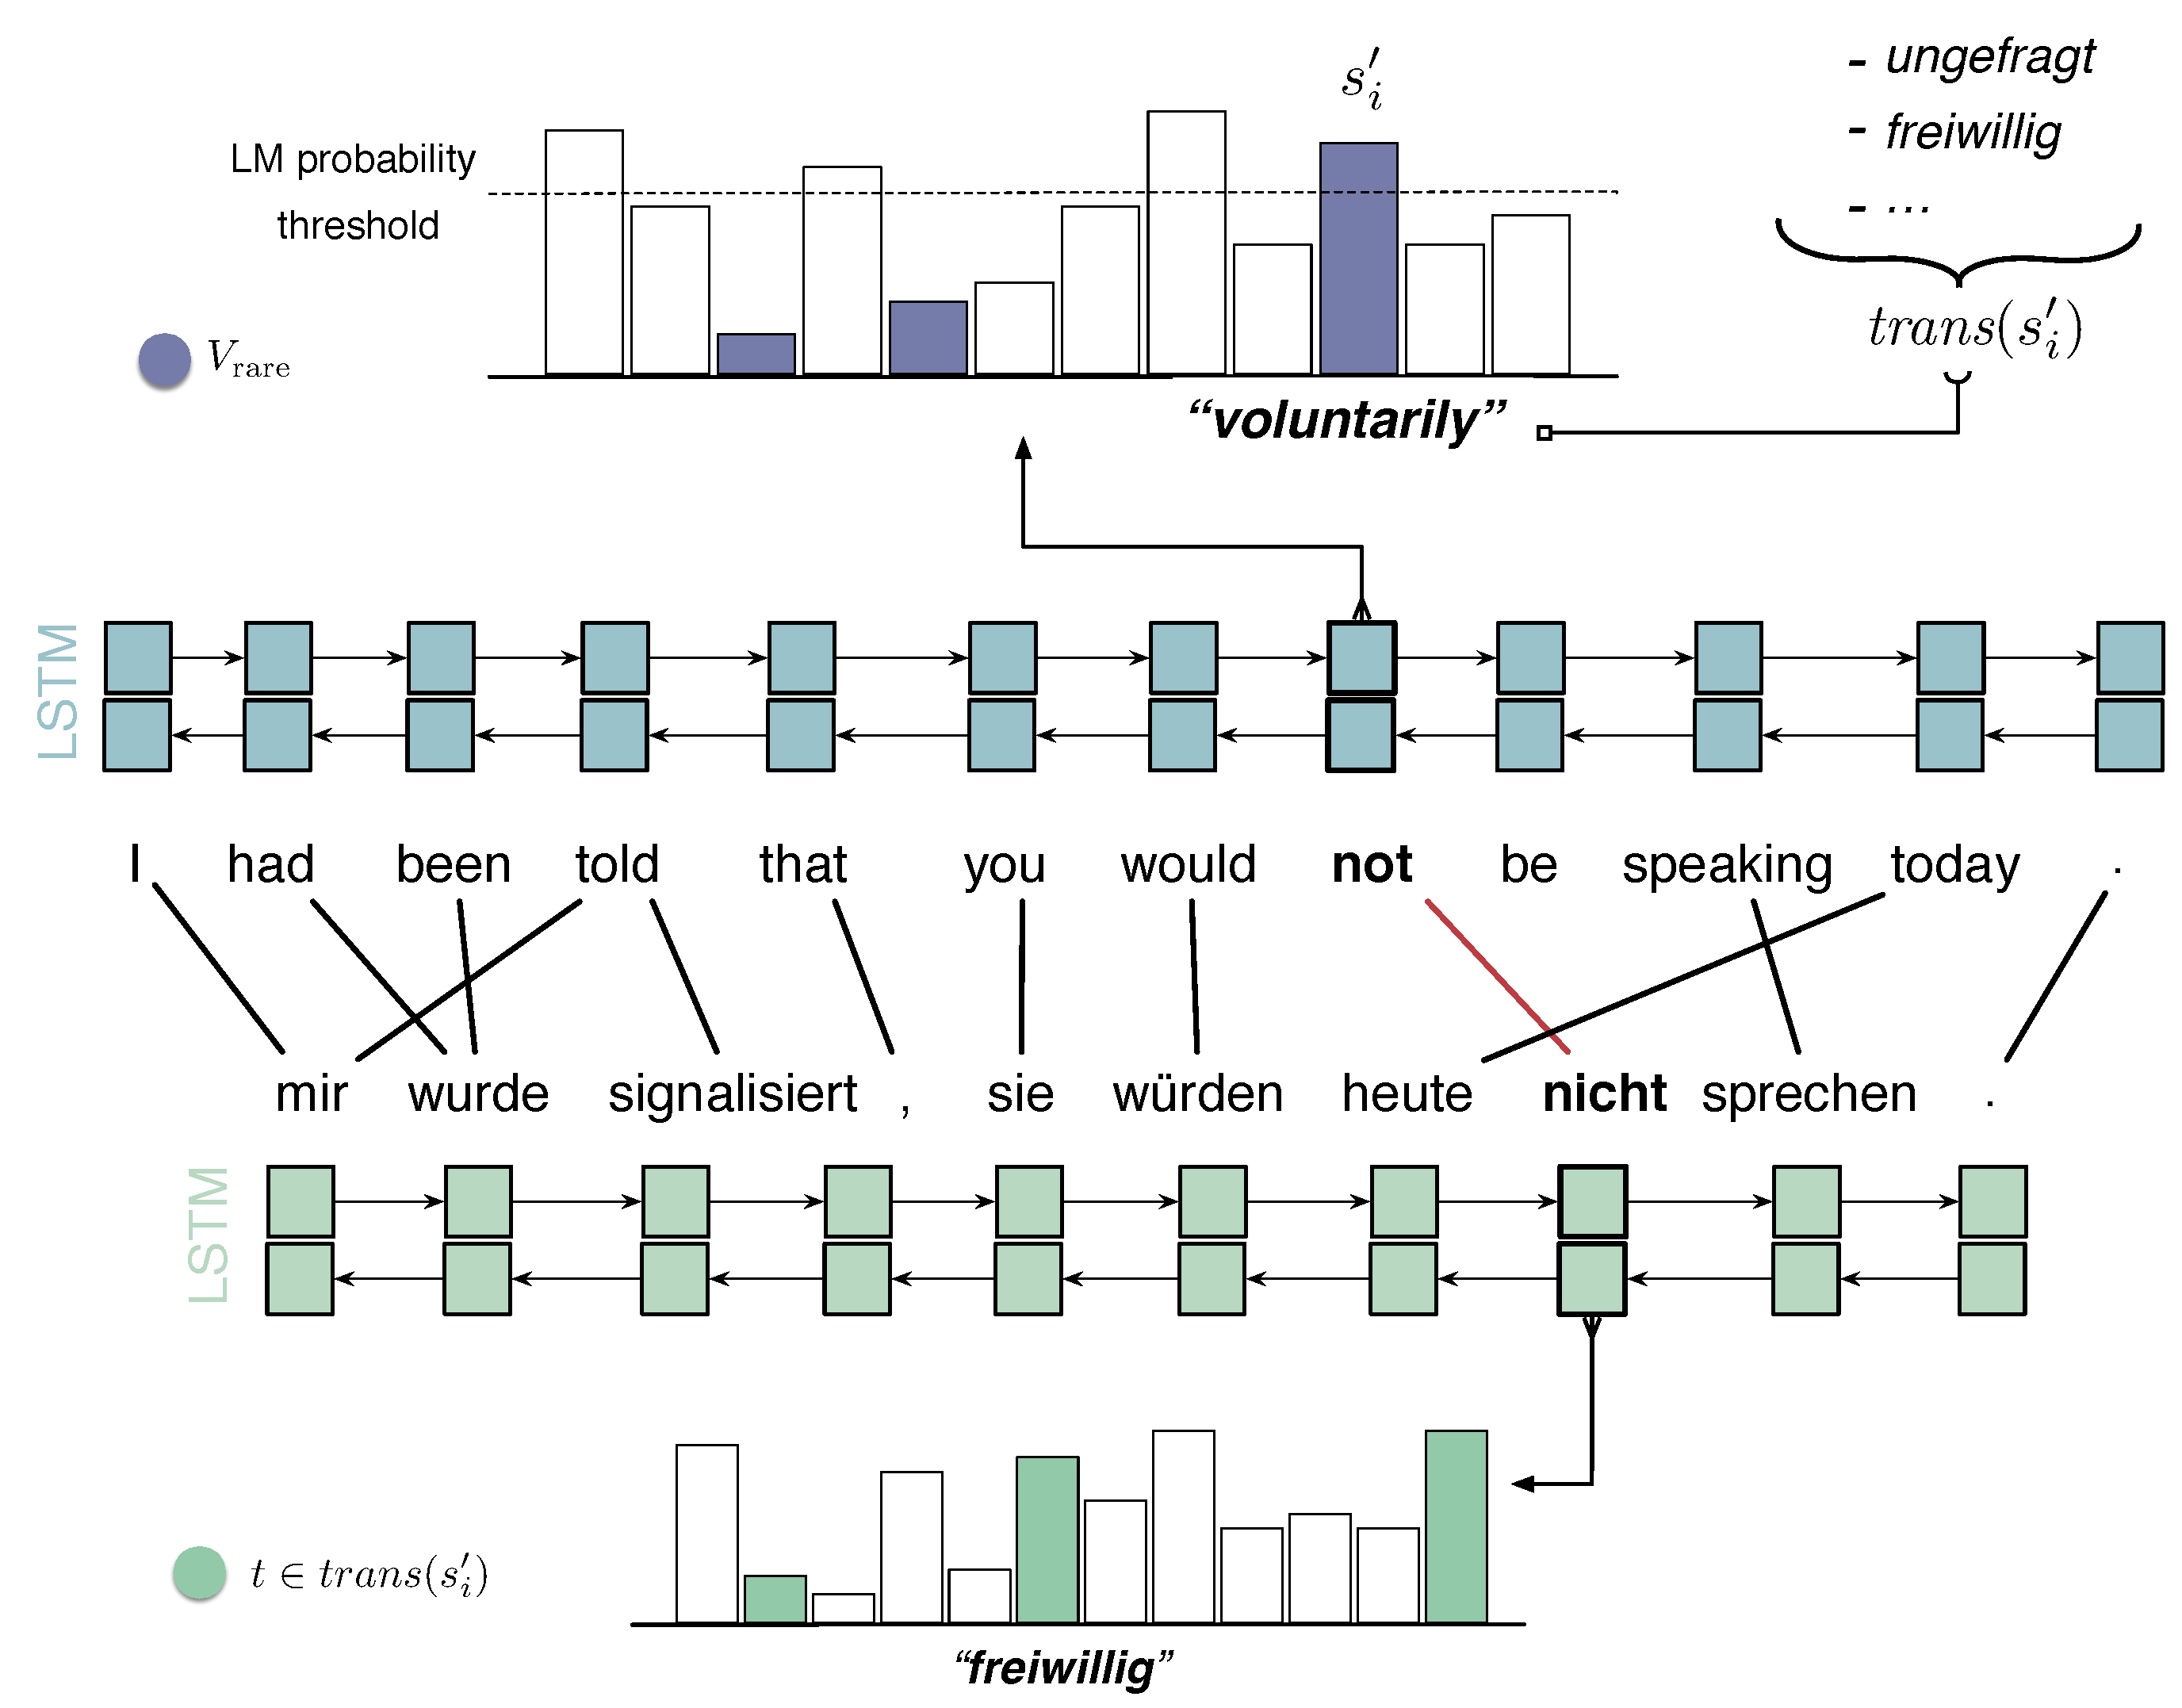
\includegraphics[width=0.88\linewidth]{04-research-02/figs/dta.pdf}
\caption{A visual representation of our proposed mechanism for generating new sentence pairs.}
\label{tdaposter}
\end{figure}
From the translation candidates, we choose the word that yields the most fluent sentence according to the German language model.
Therefore the word `\textit{freiwillig}' is selected to substitute `\textit{nicht}' in the German sentence.
The newly generated sentence pairs are then added to the training data. 

Table~\ref{examples} provides several examples resulting from our augmentation procedure. 
While using a large LM to substitute words with rare words mostly results in grammatical sentences, this does not mean that the meaning of the original sentence is always preserved. 
Note that meaning preservation is not an objective of the proposed approach in this section and we will explore this further in Section~\ref{tda:semantic}.  

\begin{table}[hbt!]
%\begin{minipage}[c]{0.48\linewidth}
\centering
\small
%\begin{tabularx}{\linewidth}{@{\ }l @{\ \ \ }X@{\ }}
\caption{Examples of augmented data with highlighted \underline{Original} words and \textbf{substituted} words. \label{examples}
% [$w_1$ / $w_2$] in the sentence indicates the replacement where $w_1$ is the original word and $w_2$ is substitution. 
%In the English sentence the substitution is suggested by the LM, and in the German sentence by the alignments to the English substitution. % WE SAID THIS BEFORE
}
\begin{tabularx}{\linewidth}{l@{\hskip 0.2in}X@{\hskip 0.2in}X}
 \toprule
 & \textbf{Original sentence pair} & \textbf{Synthetic sentence pair} \\
 \midrule
(a) & \textsc{src:} I had been told that you would \underline{not} be speaking today. &  \textsc{src:} I had been told that you would \textbf{voluntarily} be speaking today. \\
 & \textsc{tgt:} mir wurde signalisiert, sie w{\"u}rden heute \underline{nicht} sprechen. & \textsc{tgt:} mir wurde signalisiert, sie w{\"u}rden heute \textbf{freiwillig} sprechen.\\
 \midrule
(b) & \textsc{src:} the present situation is \underline{indefensible} and completely unacceptable to the commission. & \textsc{src:} the present situation is \textbf{confusing} and completely unacceptable to the commission.\\
  & \textsc{tgt:} die situation sei \underline{unhaltbar} und f{\"u}r die kommission g{\"a}nzlich unannehmbar. &  \textsc{tgt:} die situation sei \textbf{verwirrend} und f{\"u}r die kommission g{\"a}nzlich unannehmbar.\\
% EXAMPLE OK
\midrule
(c) &  \textsc{src:}  \ldots agree wholeheartedly with the institution of an ad hoc delegation of parliament on the turkish \underline{prison} system. &  \textsc{src:} \ldots agree wholeheartedly with the institution of an ad hoc delegation of parliament on the turkish \textbf{missile} system.\\
 &  \textsc{tgt:} \ldots ad-hoc delegation des parlaments f{\"u}r das regime in den t{\"u}rkischen \underline{gef{\"a}ngnissen} voll und ganz zustimmen. & \textsc{tgt:} \ldots ad-hoc delegation des parlaments f{\"u}r das regime in den t{\"u}rkischen \textbf{flugwaffen} voll und ganz zustimmen.\\
\midrule
(d) & \textsc{src:} cancellation fees are \underline{not} subject to \underline{judiciary} mitigation.  &  \textsc{src:} cancellation fees are \textbf{generally} subject to \textbf{western} mitigation. \\
 &  \textsc{tgt:} stornogeb{\"u}hren unterliegen \underline{nicht} dem \underline{richterlichen} m{\"a}{\ss}igungsrecht. &  \textsc{tgt:} stornogeb{\"u}hren unterliegen \textbf{allgemein} dem \textbf{westlichen} m{\"a}{\ss}igungsrecht. \\
\bottomrule
\end{tabularx}
\end{table}

In our experiments, two translation data augmentation (TDA) setups are considered: only one word per sentence can be replaced (TDA$_{r=1}$) or multiple words per sentence can be replaced, with the condition that any two replaced words are at least five positions apart (TDA$_{r\ge1}$).
The latter incurs a higher risk of introducing noisy sentences but has the potential to positively affect more rare words within the same amount of augmented data. 
We evaluate both setups in the following section.


%

\section{Data and experimental setup} \label{tda:exp}

In this section, we describe the experimental settings.
To simulate a low-resource setting we randomly sample 10\% of the English$\leftrightarrow$German WMT15 training data and report results on newstest 2014, 2015, and 2016 \citep{bojar-EtAl:2016:WMT1}. 
For reference, we also provide the result of our baseline system on the full data.
% sentence pairs from the corpora to train the baseline and use for augmentation experiments. 

As NMT system, we use a 4-layer attention-based encoder-decoder model as described in Section~\ref{RNN} trained with hidden dimension 1000, and batch size 80 
for 20 epochs.
NMT models often limit their vocabularies to be the top $K$ most frequent words in each language because of the computationally intensive nature of the softmax.
In all experiments, the NMT vocabulary is limited to the 30K most common words in both languages.
Note that our proposed data augmentation method does not introduce new words to the vocabulary.
%
In all experiments, we preprocess source and target language data with Byte Pair Encoding (BPE) \citep{sennrich-haddow-birch:2016:P16-12} using 30K merge operations. 
In the non-label-preserving augmentation experiments, BPE is performed after data augmentation. %, which also addresses to some extent the problem of rare words. 

For the LMs needed for data augmentation, we train 2-layer LSTM networks in forward and backward directions on the monolingual data provided for the same task 
(3.5B and 0.9B tokens in English and German, respectively) 
with embedding size 64 and hidden size 128.
%
We set the rare word threshold $R$ to 100, and top $K$ words to 1000. 
These values are determined heuristically from the training data.
 %and maximum number $N$ of augmentations per rare word to 500.
%
%and the German LM to choose the optimal word translation in context.
Another question we want to investigate is whether rare word substitution is more effective in the source or the target language. 
Therefore in the experiments, we augment the source side in English$\rightarrow$German, and target side in German$\rightarrow$English translation. 
In all experiments, we use the English LM for the rare word substitutions.
Since our first approach is not label-preserving, we only perform augmentation during training and do not alter source sentences during testing.
In Section~\ref{tda:semantic}, we also alter source sentences during testing while preserving labels.


\newcommand{\sigspace}{\rule{3ex}{0pt}}
\newcommand{\sigspacehalf}{\rule{1.6ex}{0pt}}
\begin{table}
\setlength{\tabcolsep}{5pt}
\centering
\caption{\label{bleuTBdeen} Translation performance (BLEU) on German-English WMT test sets (2014, 2015, and 2016) in a simulated low-resource setting. Back-translation refers to the work of~\citet{sennrich-haddow-birch:2016:P16-11}. 
Statistically significant improvements are marked $^\blacktriangleup$ at the $p < .01$ and $^\smalltriangleup$ at the $p < .05$ level, with the first superscript referring to baseline and the second to back-translation$_{1:1}$.}
\begin{tabular}{lcllllll}
\toprule
\multicolumn{2}{c}{}    & \multicolumn{6}{c}{\textbf{De-En}} \\\cline{3-8}
\rule{0pt}{2.5ex}    \textbf{Model}   & \textbf{Data} &  \multicolumn{2}{c}{\bf WMT14} &  \multicolumn{2}{c}{\bf WMT15} &  \multicolumn{2}{c}{\bf WMT16}\\ \midrule     
Full data (ceiling)  & 3.9M &  21.1 &  & 22.0 & & 26.9  &  \\\midrule
Baseline  & 371K & 10.6 & & 11.3 & & 13.1  & \\
%
Back-translation$_{1:1}$  & 731K & 11.4 & (+0.8)$^{\blacktriangleup}$\sigspacehalf & 12.2 & (+0.9)$^{\blacktriangleup}$\sigspacehalf & 14.6 & (+1.5)$^{\blacktriangleup}$  \\
%
Back-translation$_{1:3}$  & 1.5M & 11.2 & (+0.6)\sigspace & 11.2 & (--0.1)\sigspace & 13.3 & (+0.2)\sigspace \\\midrule
%
TDA$_{r=1}$ & 4.5M  &  11.9 & (+1.3)$^{\blacktriangleup,\mhyphen}$ & 13.4 & (+2.1)$^{\blacktriangleup,\blacktriangleup}$ & 15.2 & (+2.1)$^{\blacktriangleup,\blacktriangleup}$  \\
%
TDA$_{r\ge 1}$ &  6M    &  \textbf{12.6}  & (+2.0)$^{\blacktriangleup,\blacktriangleup}$ & \textbf{13.7} & (+2.4)$^{\blacktriangleup,\blacktriangleup}$ & \textbf{15.4} & (+2.3)$^{\blacktriangleup,\blacktriangleup}$ \\
%
Oversampling & 6M & 11.9 & (+1.3)$^{\blacktriangleup,\mhyphen}$ & 12.9 & (+1.6)$^{\blacktriangleup,\smalltriangleup}$ & 15.0 & (+1.9)$^{\blacktriangleup,\mhyphen}$  \\
\bottomrule
\end{tabular}
\end{table}


\begin{table}
\setlength{\tabcolsep}{5pt}
\centering
\caption{\label{bleuTBende} Translation performance (BLEU) on English-German WMT test sets (2014, 2015, and 2016) in a simulated low-resource setting. Back-translation refers to the work of~\citet{sennrich-haddow-birch:2016:P16-11}. 
Statistically significant improvements are marked $^\blacktriangleup$ at the $p < .01$ and $^\smalltriangleup$ at the $p < .05$ level, with the first superscript referring to baseline and the second to back-translation$_{1:1}$.}
\begin{tabular}{lcllllll}
\toprule
\multicolumn{2}{c}{}    & \multicolumn{6}{c}{\textbf{En-De}}  \\\cline{3-8}
\rule{0pt}{2.5ex} \textbf{Model}   & \textbf{Data} &  \multicolumn{2}{c}{\bf WMT14} &  \multicolumn{2}{c}{\bf WMT15} &  \multicolumn{2}{c}{\bf WMT16}\\ \midrule     
Full data (ceiling)  & 3.9M &   17.0 & & 18.5 & & 21.7 & \\\midrule
Baseline  & 371K   & 8.2 & & 9.2 & & 11.0 & \\
%
Back-translation$_{1:1}$  & 731K &  9.0 & (+0.8)$^{\blacktriangleup}$\sigspacehalf & 10.4 & (+1.2)$^{\blacktriangleup}$\sigspacehalf & 12.0 & (+1.0)$^{\blacktriangleup}\sigspacehalf$ \\
%
Back-translation$_{1:3}$  & 1.5M & 7.8 & (--0.4)\sigspace & 9.4 & (+0.2)\sigspace & 10.7 & (--0.3)\sigspace \\\midrule
%
TDA$_{r=1}$ & 4.5M  &  10.4 & (+2.2)$^{\blacktriangleup,\blacktriangleup}$  & 11.2 & (+2.0)$^{\blacktriangleup,\blacktriangleup}$ & 13.5 & (+2.5)$^{\blacktriangleup,\blacktriangleup}$  \\
%
TDA$_{r\ge 1}$ &  6M    & \textbf{10.7} & (+2.5)$^{\blacktriangleup,\blacktriangleup}$  & \textbf{11.5} & (+2.3)$^{\blacktriangleup,\blacktriangleup}$ & \textbf{13.9} & (+2.9)$^{\blacktriangleup,\blacktriangleup}$ \\
%
Oversampling & 6M & 9.7 & (+1.5)$^{\blacktriangleup,\smalltriangleup}$ & 10.7 & (+1.5)$^{\blacktriangleup,\mhyphen}$ & 12.6 & (+1.6)$^{\blacktriangleup,\mhyphen}$ \\
\bottomrule
\end{tabular}
\end{table}


We also compare our approach to~\citet{sennrich-haddow-birch:2016:P16-11} by back-translating monolingual data and adding it to the parallel training data.
Specifically, we back-translate sentences from the target side that are not included in our low-resource baseline with two settings: keeping a one-to-one ratio of back-translated %pseudo 
versus original data (\mbox{$1:1$}) following the authors' suggestion, or using three times more back-translated data (\mbox{$1:3$}).
% in their paper and kept the ratio of the back-translated and original parallel corpora one-to-one.
We measure translation quality by single-reference case-insensitive BLEU \citep{Papineni2001} computed with the \code{multi-bleu.perl} script from Moses.


\section{Results} \label{tda:results}

In this section, we discuss the results on the translation task and evaluate the effectiveness of our approach in a simulated low-resource NMT scenario.
We repeat the sampling and substitution step iteratively until we reach the desired corpus size for each experiment. 
In our various experiments, we successfully augment between $72\%$ to $81\%$ of targeted rare words. 
All translation results are displayed in Table~\ref{bleuTBdeen} and Table~\ref{bleuTBende} for German$\rightarrow$English and English$\rightarrow$German experiments, respectively. 
%shows the results for English$\leftrightarrow$German translation on different test sets. 

First, we observe that the low-resource baseline performs much worse than the full data system,
re-iterating the importance of sizable training data for NMT. %, but it is well performing proportional to the training size.
Next, we observe that both back-translation and our proposed TDA method significantly improve translation quality. However, TDA obtains the best results overall and significantly outperforms back-translation for all test sets. % (note that increasing the amount of back-translated data does not improve but actually worsen the results obtained)
This is an important finding considering that our method involves only minor modifications to the original training sentences and does not involve any costly translation process, while the back-translation approach augments with novel target sentences.
%
Improvements are consistent across both translation directions, %Similar trends appear in both translation directions, 
regardless of whether rare word substitutions are applied to the source or to the target side.
We also observe that altering multiple words in a sentence performs slightly better than altering only one word.
This indicates that addressing more rare words is preferable even though the augmented sentences are more likely to be noisy.  

To verify that the gains are actually due to the rare word substitutions and not just to the repetition of part of the training data, we perform a final experiment where each sentence pair selected for augmentation is added to the training data \textit{unchanged} (Oversampling row in Tables~\ref{bleuTBdeen} and~\ref{bleuTBende}). 
Surprisingly, we find that this simple form of sampled data replication outperforms both baseline and back-translation systems,\footnote{Note that this effect cannot be achieved by simply continuing the baseline training for up to 50 epochs.} while TDA\textsubscript{$_{r\ge 1}$} remains the best performing system overall.

\begin{table}[htb!]
\centering
\setlength{\tabcolsep}{4pt}
\caption{Average length of German$\rightarrow$English translation systems, along with the average length of human reference translations (bottom line). Predominantly, we favour longer translations that are close to human reference translations, i.e., models with higher \% Ref ratio.\label{sentlen1} }
\begin{tabular}{lcccc}
\toprule
& \multicolumn{3}{c}{ \textbf{De-En}}   \\
\cline{2-4}
\rule{0pt}{2.5ex}     & \bf WMT14 & \bf WMT15 & \bf WMT16 & \bf  \%Ref    \\
 \midrule
Baseline & 19.9 & 19.2 & 19.9 & 0.88  \\
TDA$_{r= 1}$ & 21.4 & 20.4 & 21.2 & \textbf{0.94} \\
%\rule{0pt}{2.5ex} 
TDA$_{r\ge 1}$ & 21.0 & 20.0 & 20.8 & 0.92  \\
\hdashline
%\rule{0pt}{2.5ex} 
Reference & 23.0 & 22.2 & 21.9 & 1.00  \\
\bottomrule
\end{tabular}
\end{table}
\begin{table}[htb!]
\centering
\setlength{\tabcolsep}{4pt}
\caption{Average length of English$\rightarrow$German translation systems, along with the average length of human reference translations (bottom line). Predominantly, we favour longer translations that are close to human reference translations, i.e., models with higher \% Ref ratio.\label{sentlen2} }
\begin{tabular}{lcccc}
\toprule
&  \multicolumn{3}{c}{ \textbf{En-De} }   \\
\cline{2-4} 
\rule{0pt}{2.5ex}     & \bf WMT14 & \bf WMT15 & \bf WMT16 & \bf  \%Ref    \\
 \midrule
Baseline  & 19.8 & 19.4 & 18.9 & 0.91 \\
TDA$_{r= 1}$ &  20.5 & 20.2 & 19.9 & \textbf{0.95} \\
%\rule{0pt}{2.5ex}  
TDA$_{r\ge 1}$  & 20.7 & 20.0 & 19.8 & \textbf{0.95} \\
\hdashline
%\rule{0pt}{2.5ex} 
Reference & 21.4 & 20.8 & 21.6 & 1.00 \\
\bottomrule
\end{tabular}
\end{table}
%
We also observe that the system trained on our augmented data tends to generate longer translations, which is favoured. % than the baseline. 
Tables~\ref{sentlen1} and~\ref{sentlen2} provide the average length of the translation outputs of different systems, along with the average length of human reference translations.
Averaging over all test sets and language pairs, the length of translations generated by the baseline is 0.89 of the average reference length, while for TDA\textsubscript{$_{r=1}$} and TDA\textsubscript{$_{r\ge 1}$} it is 0.94 and 0.93, respectively.
%during testing. 
We attribute this effect to the ability of the TDA-trained system to generate translations for rare words that were left untranslated by the baseline system.


\begin{figure}
\centering
\begin{tikzpicture}[shorten >=1pt, node distance=2.5cm,scale=1]
\pgfplotstableread{
X   Gp   Name        generated     rare         notrareanymoreGen   notrareanymoreNotGen 
8   baseline   14    604   3389  0   0
7   TDA test 2114   3389     2082  32   
5   baseline   15    480   2528    0    0
4   TDA   test    1522   2528    1422    100
2   baseline   16    627   3146   0    0
1   TDA   test  2072   3146    1998  70
}\datatable
% 2014 (33). 2015 (29). 2016 (19)
\begin{axis}[
    %axis lines*=left, ymajorgrids,
     width=8.5cm, height=6.5cm,
     xmin=0,
     %xbar stacked,
     xbar,
     xmax = 3500, 
     bar width=13pt,
     bar shift=0pt,
     ytick=data,
     reverse legend,
         xtick={1000, 2000, 3000},
     %axis y line*=right,
     yticklabels from table={\datatable}{Gp},
         ytick style={draw=none},
     %ylabel = test2014 \hspace{1em} test2015  \hspace{1em} test2016,
     legend style={at={(0.42,-0.15)},anchor=north, draw=none, /tikz/every even column/.append style={column sep=5pt}}, 
     legend image code/.code={%
             \draw[#1] (0cm,-0.1cm) rectangle (0.3cm,0.1cm);
        },
     legend cell align=left
]

\addplot [fill=blu, fill opacity=1] table [y=X, x=rare] {\datatable};  \addlegendentry{{Words in $V_R \cap V_{ref}$ not generated during translation}} %Rare words that are generated during translation}}
\addplot [fill=gr, fill opacity=1] table [y=X, x=generated] {\datatable}; \addlegendentry{{Words in $V_R \cap V_{ref}$ generated during translation }}
\end{axis}

\begin{axis}[
    %axis lines*=left, ymajorgrids,
    width=8.5cm, height=6.5cm,
    xmin=0,
    xbar stacked,
    xmax = 3000,
    bar width=13pt,
    ytick=data,
    axis y line*=right,
    y tick label style={rotate=90} ,
     yticklabels from table={\datatable}{Name},
    xticklabels=\empty,
    xtick=\empty,
    ytick style={draw=none},
     legend style={at={(0.35,-0.345)},anchor=north, draw=none, /tikz/every even column/.append style={column sep=5pt}}, 
     legend image code/.code={%
             \draw [pattern=north east lines](0cm,-0.1cm) rectangle (0.3cm,0.1cm);
        },
     legend cell align=left,
]
\addplot [fill=red, fill opacity=0,forget plot] table [y=X, x=notrareanymoreNotGen] {\datatable};
\addplot [pattern=north east lines] table [y=X, x=notrareanymoreGen] {\datatable}; \addlegendentry{Words in $V_R \cap V_{ref}$ affected by augmentation}

\end{axis}
\end{tikzpicture}
\caption{Effect of TDA on the number of unique rare words generated during De$\rightarrow$En translation. $V_R$ is the set of rare words targeted by TDA\textsubscript{$_{r\ge 1}$} and $V_{ref}$ the reference translation vocabulary.} % The hatched pattern indicates words that are not rare anymore i.e., were augmented in the training data.}
\label{rarewordfreqs}
\end{figure}

\section{Further analysis}  \label{tda:analysis} 

In this section, we further analyze our findings and discuss the results of our proposed models.
Our goal is to understand the impact of the introduced diverse contexts on the learning capabilities of the neural translation model. 

\begin{table}[p]
%\begin{minipage}[c]{0.48\linewidth}
\rotatebox{90}{
\begin{minipage}{\textheight}
\begin{center}
%\begin{tabularx}{\linewidth}{@{\ }l @{\ \ \ }X@{\ }}
\caption{An example from WMT14 illustrating the effect of augmenting rare words on generation at test time. 
The translation of the baseline does not include the rare word \textit{centimetres}, however, the translation of our TDA model generates the rare word and produces a more fluent sentence. Instances of the augmentation of the word \textit{centimetres} in training data are also provided. \label{transex}}
\begin{tabularx}{0.8\textheight}{l@{\hskip 0.02in}X@{\hskip 0.2in}X}
% \multirow{2}{*}{(a)} & \textsc{src:}  &  \textsc{src:}  \\
 %& \textsc{tgt:}  &  \textsc{tgt:}  \\
 %\multicolumn{3}{l}{ } \\
  \multicolumn{3}{l}{\textit{Example from WMT14}}  \\
 \toprule
\textsc{src} & \multicolumn{2}{l}{der tunnel hat einen querschnitt von 1,20 meter h{\"o}he und 90 \underline{zentimeter} breite.}\\ 
\textsc{ref}   & \multicolumn{2}{l}{the tunnel has a cross-section measuring 1.20 metres high and 90 \underline{centimetres} across.} \\
%\specialrule{.05em}{0em}{0em} 
Baseline  & \multicolumn{2}{l}{the wine consists of about 1,20 m and 90 of the canal.} \\
TDA\textsubscript{$_{r\ge 1}$}  & \multicolumn{2}{l}{the tunnel has a \texttt{unk} measuring meters 1.20 metres high and 90 \textbf{centimetres} wide.} \\
\bottomrule
% & $\bullet$ various shopping venues , countless bars and restaurants and a nightclub are to be found in the vicinity ( 100 [m / \textbf{centimetres}]  radius ) .\
\noalign{\vskip 5mm} 
 \multicolumn{3}{l}{ \textit{Examples from the training data displaying augmentations for the word \textbf{`centimetres'}}} \\
\toprule
& Original data & Augmented data \\ 
\midrule
(a) & the average speed of cars and buses is therefore around 20 \underline{kilometres}  per hour.  & the average speed of cars and buses is therefore around 20 \textbf{centimetres} per hour. \\
 \hdashline
(b) & grab crane in special terminals for handling capacities of up to 1,800 \underline{tonnes} per hour.  &  grab crane in special terminals for handling capacities of up to 1,800 \textbf{centimetres} per hour.\\ 
  \hdashline
(c) &  all suites and rooms are very spacious and measure between 50 and 70 \underline{m}. & all suites and rooms are very spacious and measure between 50 and 70 \textbf{centimetres}. \\ 
  \hdashline
(d) &   all we have to do is lower the speed limit everywhere to five \underline{kilometers} per hour. &  all we have to do is lower the speed limit everywhere to five \textbf{centimetres} per hour.\\ 
  \hdashline
(e) &  just 9.5 litres of water per minute flow through the innovative \texttt{unk} shower system, whereas the hansgrohe \texttt{unk} 85 green hand spray manages with only six \underline{litres} per minute. & just 9.5 litres of water per minute flow through the innovative \texttt{unk} shower system, whereas the hansgrohe \texttt{unk} 85 green hand spray manages with only six \textbf{centimetres} per minute.  \\ 
\bottomrule
\end{tabularx}
\end{center}
\end{minipage}
}
\end{table}


\subsection{Target words} 
A desired effect of our method is to increase the number of correct rare words generated by the NMT system at test time. 
To illustrate the impact of augmenting the training data by creating contexts for rare words on the \textit{target} side, Table~\ref{transex} provides an example for German$\rightarrow$English translation. 

We see that the baseline model is not able to generate the rare word \textit{`centimetres'} as a correct translation of the German word \textit{`zentimeter'}. However, this word is not rare in the training data of the TDA\textsubscript{$_{r\ge 1}$} model after our augmentation and is generated during translation. Table~\ref{transex} also provides several instances of augmented training sentences targeting the word \textit{`centimetres'}. Note that even though some augmented sentences are rather unusual (e.g., \textit{`the speed limit is five centimetres per hour'}), the NMT system still benefits from the new context for the rare word and is able to generate it during testing.

Figure~\ref{rarewordfreqs} demonstrates that this is indeed the case for many words: the number of rare words occurring in the reference translation ($V_R \cap V_{ref}$) is three times larger in the TDA system output than in the baseline output. 
%Figure~\ref{rarewordfreqs} shows the number of words generated during translations in different test sets for the baseline and TDA\textsubscript{multiple} system. 
One can also see that this increase is a direct effect of TDA
as most of the rare words are not `rare' anymore in the augmented data, i.e., they were augmented sufficiently often to occur more than 100 times (see the hatched pattern in Figure~\ref{rarewordfreqs}).
%We observe that the generation of rare words increases in our model in comparison with the baseline.
%This indicates that by having more instances of words in the training data, the model tends to use these words more during the translation process.
Note that in our experiments, we did not use any information from the evaluation sets.



\subsection{Source words}  

To gauge the impact of augmenting the contexts for rare words on the \textit{source} side, we examine normalized attention scores of these words before and after augmentation. When translating English$\rightarrow$German 
with our TDA model, the attention scores for rare words on the source side are on average 8.8\% higher than when translating with the baseline model. This suggests that having more accurate representations of rare words increases the model's confidence to attend to these words when encountered during test time.


\subsection{Negative examples}  

Table~\ref{tdaexampleswrong} provides examples of cases where augmentation results in incorrect sentences. 
In the first example, the sentence is ungrammatical after substitution (\textit{`of / yearly'}), which can be the result of choosing substitutions with low probabilities from the English LM $\topk$ suggestions. 


\begin{table}[p]
\rotatebox{90}{
\begin{minipage}{\textheight}
\begin{center}
\caption{Examples of incorrectly augmented data with highlighted \underline{Original} words and \textbf{substituted} words. \label{tdaexampleswrong}}
\begin{tabularx}{0.8\linewidth}{l@{\hskip 0.07in}X@{\hskip 0.2in}X}
 \toprule
  & Original sentence pair & Synthetic sentence pair \\
\midrule
% \multirow{2}{*}{(a)} & \textsc{src:}  &  \textsc{src:}  \\
 %& \textsc{tgt:}  &  \textsc{tgt:}  \\
 %\multicolumn{3}{l}{ } \\
(a) & \textsc{src:} registered users will receive the \texttt{unk} newsletter free \underline{of} charge.&  \textsc{src:}  registered users will receive the \texttt{unk} newsletter free \textbf{yearly} charge. \\
 & \textsc{tgt:} registrierte user erhalten zudem regelm{\"a}{\ss}ig \underline{den} markenticker newsletter.  &  \textsc{tgt:}  registrierte user erhalten zudem regelm{\"a}{\ss}ig \textbf{j{\"a}hrlich} markenticker newsletter.  \\
\noalign{\vskip 2mm}   \hdashline
 \textsc{Problem:} & \multicolumn{2}{l}{ \textit{Substitution results in syntactically incorrect source and target sentences.} } \\
 \midrule
(b) & \textsc{src:}  the personal contact is \underline{essential} to us. &  \textsc{src:}  the personal contact is \textbf{entrusted} to us. \\
                      & \textsc{tgt:} pers{\"o}nliche kontakt ist uns sehr \underline{wichtig}.  &  \textsc{tgt:} pers{\"o}nliche kontakt ist uns sehr \textbf{betraut}. \\
\noalign{\vskip 2mm}   \hdashline
 \textsc{Problem:} & \multicolumn{2}{l}{ \textit{The German sentence is grammatically incorrect.} } \\
  \midrule
(c) & \textsc{src:} \texttt{unk}  \texttt{unk} wishes you very \underline{pleasant} holiday. &  \textsc{src:}  \texttt{unk}  \texttt{unk} wishes you very \textbf{crazy} holiday. \\
 & \textsc{tgt:}  \texttt{unk} \texttt{unk} w{\"u}nscht ihnen einen \underline{erholsamen} urlaub.  &  \textsc{tgt:} \texttt{unk}  \texttt{unk} w{\"u}nscht ihnen einen \textbf{verr{\"u}ckt} urlaub. \\
\noalign{\vskip 2mm}    \hdashline
 \textsc{Problem:} &  \multicolumn{2}{l}{\textit {German substitution has the wrong inflection.}} \\
 \midrule
(d) & \textsc{src:} \underline{consumers} are currently being \underline{deliberately} misled. &  \textsc{src:}  \textbf{schools} are currently being \textbf{widely} misled. \\
 & \textsc{tgt:}  \underline{die} verbraucher werden gegenw{\"a}rtig \underline{bewusst} get{\"a}uscht. &  \textsc{tgt:}  \textbf{schulen} verbraucher werden gegenw{\"a}rtig \textbf{weithin} get{\"a}uscht. \\
\noalign{\vskip 2mm}    \hdashline
 \textsc{Problem:} & \multicolumn{2}{l}{\textit{Substituted with the wrong German word because of wrong alignment.} } \\
\bottomrule
\end{tabularx}
\end{center}
\end{minipage}
}
\end{table}

Errors can also occur during translation selection, as in the second example where \textit{`betraut'} is an acceptable translation of \textit{`entrusted'} but would require a rephrasing of the German sentence to be grammatically correct.
Problems of this kind can be attributed to the German LM, but also to the lack of a more suitable translation in the lexicon extracted from the bitext.
Interestingly, this noise seems to affect NMT only to a limited extent.

\subsection{Word segmentation} 
BPE \citep{sennrich-haddow-birch:2016:P16-12} is an essential preprocessing step in NMT to address the problem of rare and unknown words in the training data and we use it in all experiments. 
Although crucial, it is not very effective in a low-resource setting \citep{ngo-etal-2019-overcoming}.
We suspect that this is caused by the scarcity of data, which results in inaccurate word splits with possibly rare subword units.
This can be observed in the example in Table~\ref{transex}. 
In the experiments, the English and German words \textit{`centi$\mid$metres'} and \textit{`zenti$\mid$meter'} are both split into two subword units. Still, the baseline model fails to translate it correctly.
This further stresses the importance of data augmentation with diverse contexts. 
Even though BPE segmentation is successful in rare word translations, our proposed approach yields additional improvements.

\section{Meaning-Preserving augmentation}  \label{tda:semantic}

In the previous section, we proposed a model with a weak notion of label preservation that allows modifying both source and target sentences at the same time as long as they remain translations of each other. 
As a result, we alter and augment the training data, and the test data remains unchanged. 
%
This approach improves translation quality by better translating rare words because of the additional contexts during training. 
However, it does not address the problem of translating out-of-vocabulary (OOV) words during testing.
To specifically target OOV words at test time, we propose a stronger notion of label preservation to only alter source sentences with paraphrases. 
Note that at test time, we only have access to source sentences and keep the reference sentences unchanged. 

In this section, we investigate how we can benefit from external lexical resources to address the problem of translating unknown words. 
We define OOV as words not listed in the 30k most common words in source and target vocabulary. 
While BPE is an effective approach in addressing the OOV translation problem, we do not use it in these experiments.
To benefit from external knowledge resources, we substitute OOVs with synonym words obtained from these resources that exist in our vocabulary. 
%
We experiment with three different resources to alter source sentences with paraphrases:

\subparagraph{PPDB} proposed by~\citet{ganitkevitch-etal-2013-ppdb}. This Paraphrase Database is an automatically extracted database from parallel corpora containing millions of paraphrases in multiple languages.

\subparagraph{Wordnet} proposed by~\citet{miller1995wordnet}. WordNet is a manually created large lexical database of English and includes relations between words and groups of cognitive synonyms. We use GermaNet \citep{hamp-feldweg-1997-germanet,HENRICH10.264} which is a lexical-semantic resource similar to Wordnet for the German language.

\subparagraph{CBOW} embeddings proposed by~\citet{mikolov2013distributed}. We use the Continuous Bag of Words (CBOW) model to identify the words most similar to each OOV word and interpret that as the synonym. %In contrast to the previous two resources, this method is trained using context. % and as a result provides context-aware synonyms. 
\subparagraph{HTLE} embeddings proposed in Chapter~\ref{chapter:research-01}. We use the multiple topic-sensitive representations per word to identify synonyms according to the context of the word. 
In contrast to the previous resources, this method provides context-sensitive synonyms which means the same word in different contexts has different synonym substitutions. 

\gap 

We substitute the OOV words in source sentences with synonyms that already exist in the NMT vocabulary. % acquired from the parallel training data.  
An example of the substitution is shown in Table~\ref{augwnexample} where the original word `\textit{fateful}' is OOV and is replaced by the \texttt{unk} symbol in the original training data.
%
%Here the word \textit{fateful} does not exist in the limited source vocabulary, and 
Each paraphrase resource suggests a substitution for the target word in the sentence. % that are different at times. 
%PPDB and Wordnet have fix suggestions for each word.
%However, the CBOW embedding uses the local context window and as a result, provides a list of most similar words specific to that context. 
We also experiment with targeting low-frequency words in the test data. 
Similar to OOVs, we substitute words that are rare in our training data (frequencies less than 100) with synonyms during test time. 

\begin{table}[htb!]
\small
\centering
\begin{tabular}{l l}
\toprule
 {original src} & {He said Lamb made the \textit{fateful} 911 call sometime after that.} \\ 
 {NMT input} & {He said Lamb made the \texttt{[unk]} 911 call sometime after that.} \\ \midrule
 +PPDB   & {He said Lamb made the \textbf{disastrous} 911 call sometime after that.}  \\
+Wordnet &  {He said Lamb made the \textbf{fatal} 911 call sometime after that.}   \\
+CBOW &  {He said Lamb made the \textbf{tragic} 911 call sometime after that.}  \\
+HTLE &  {He said Lamb made the \textbf{critical} 911 call sometime after that.}  \\
\bottomrule
\end{tabular}
 \caption{Examples of paraphrase modification. The out-of-vocabulary word \textit{fateful} in the source sentence is substituted with synonyms obtained from different lexicon resources. \label{augwnexample}}
\end{table}

Tables~\ref{semdeen} and~\ref{semende} provide the results for the translation of German$\rightarrow$English and English$\rightarrow$German, respectively.  
Note that the HTLE embeddings are available only in English and so we only use this approach in the English$\rightarrow$German translation experiments to augment English sentences on the source side.
%
Overall the results show improvements over the baseline. 
BLEU scores using PPDB and Wordnet are very similar for all experiments. %and are very close to the baseline results. 
Improvements using CBOW and HTLE are also similar, however, HTLE is the most effective method out of the four approaches.
This indicates, to a certain degree, the importance of context-aware substitutions in data augmentation.

\begin{table}[htb!]
\centering
\caption{Translation performance (BLEU) on German-English WMT news test sets (2014, 2015, and 2016). \texttt{OOV} signifies out-of-vocabulary words. \texttt{rare} words are selected with the frequency threshold of 100. \label{semdeen}}
\begin{tabular}{lllcccccc}
\toprule
   & & & \multicolumn{3}{c}{\textbf{De-En}}  \\\cline{4-6} 
\rule{0pt}{2.5ex} \textbf{Model} & \textbf{+lexical DB} & \textbf{Target}  & \bf WMT14 &  \bf WMT15 &  \bf WMT16 \\      
 \midrule
Baseline &  &  &    19.3 &   20.1 &  24.9   \\ \midrule
\multirow{4}{*}{Subs}  & {PPDB}  & \texttt{OOV} & 21.2 & 22.2 & 26.9 \\
& {GermaNet}   & \texttt{OOV}  & 20.3 & 21.9 & 25.2 \\
& {CBOW}   & \texttt{OOV}  & 21.2 & 22.4& 27.0 \\
\midrule
\multirow{4}{*}{Subs} & {PPDB}   & \texttt{OOV} + \texttt{rare}   & 21.3 & 22.3 & 26.9 \\
& {GermaNet}   & \texttt{OOV} + \texttt{rare}     & 20.5 & 22.0 & 25.4 \\
& {CBOW}   & \texttt{OOV} + \texttt{rare}  & \bf 21.4 & \bf 22.5& \bf 27.2 \\
\bottomrule
\end{tabular}
\end{table}
\begin{table}[htb!]
\centering
\caption{Translation performance (BLEU) on English-German WMT news test sets (2014, 2015, and 2016). \texttt{OOV} signifies out-of-vocabulary words. \texttt{rare} words are selected with the frequency threshold of 100. \label{semende}}
\begin{tabular}{lllccc}
\toprule
   & & & \multicolumn{3}{c}{\textbf{En-De}}   \\\cline{4-6} 
\rule{0pt}{2.5ex} \textbf{Model}  & \textbf{+lexical DB} & \textbf{Target} &  \bf WMT14 &  \bf WMT15 &  \bf WMT16 \\      
 \midrule
Baseline  & & & 15.9 &  17.6 &  20.0       \\ \midrule
\multirow{4}{*}{Subs} & {PPDB} & \texttt{OOV}     & 17.2 &  	18.5   	 & 21.8   \\
& {Wordnet}& \texttt{OOV}      & 17.2 &  	18.5   	& 21.7 \\
& {CBOW}& \texttt{OOV}      & 17.3 &  	18.6   	& 22.0 \\
& {HTLE}   & \texttt{OOV}  & 17.5 & 18.6 & 22.2 \\ \midrule
\multirow{4}{*}{Subs} & {PPDB}  & \texttt{OOV} + \texttt{rare}    & 17.2 &  	18.7   	 & 21.9  \\
& {Wordnet} & \texttt{OOV} + \texttt{rare}     & 17.1 &  	18.5   	& 21.8  \\
& {CBOW} & \texttt{OOV} + \texttt{rare}     & 17.4 &  	18.7   	& 22.2  \\
& {HTLE}   & \texttt{OOV} + \texttt{rare}  & \bf 17.9 &  	\bf 19.1   	& \bf 22.5  \\
\bottomrule
\end{tabular}
\end{table}

Finally, we look into the rate a neural model generates the \texttt{unk} symbol before and after augmentation.
When a source sentence contains several rare and OOV words, the translation model tends to use the \texttt{unk} symbol to represent these words. 
As a result, the model performs poorly and produces several \texttt{unk} symbols in the translation output.
We investigate the fluency of the translation outputs by observing the rate of the generation of the \texttt{unk} symbol.
We observe that in our experiments the number of \texttt{unk} symbols generated in the translation output drops. 
Table ~\ref{unkaveaug} provides statistics on the generation of  \texttt{unk} token. 
Surprisingly, the significant differences in the number of \texttt{unk} symbols in the translation outputs are not entirely reflected in the BLEU scores. 

\begin{table}
\centering
\caption{The impact of paraphrase augmentation on the generation of \texttt{unk} tokens in the translation output. Reductions are computed in comparison with the baseline model. Lower number of \texttt{unk}s is better.  \label{unkaveaug} }
\begin{tabular}{l|c|cccc}
%\toprule
& Baseline & PPDB & Wordnet & CBOW & HTLE \\ \midrule
Number of \texttt{unk}s & 4931 & 4851 & 4857 & 3018 & \bf 3003 \\
Reduction in number of \texttt{unk}s & - & 1.62$\%$ & 1.5$\%$ & 38.8$\%$ & \bf 39.1$\%$ \\
%\bottomrule
\end{tabular}
\end{table}


\section{Conclusion} \label{tda:conc}

In this chapter, we investigated the impact of diverse contexts on the translation of rare words.
The quality of an NMT system depends substantially on the availability of sizable parallel corpora, which is only available for a limited number of languages and domains.
%For low-resource language pairs, this is not the case, and it results in poor translation quality. 
The translation is particularly erroneous for low-frequency words; with only a few instances in the training data, the model has difficulties learning to translate these words. 
While the challenges of translating low-resource language pairs have been studied extensively, the impact of artificially generated contexts on the translation quality of words has hardly been studied. 
We addressed this issue in this chapter and investigated the effect of additional context in learning word translations, by asking:
 
\begin{enumerate}[label=\textbf{RQ2.\arabic* },wide = 0pt, leftmargin=2em]
\setlength\itemsep{1em}
\item \acl{rq:tda1}

\medskip

\noindent  Our experiments showed that by providing more diverse contexts for rare words, we improve the estimation of the model and subsequently increase the number of times the model generates these words correctly. 
We have proposed an effective approach to augment the training data of neural machine translation for low-resource language pairs. 
We generated new sentence pairs containing rare words in new contexts by leveraging language models trained on large amounts of monolingual data.
Our approach augments the data by diversifying the sentences of the parallel corpora, changing both source and target sentences.
We showed that this approach leads to generating rare words more often during translation and thus improves translation quality. 
%Our analysis further stresses that poor translation quality of rare words is a result of a lack of diverse training examples. 
We observed substantial improvements in simulated low-resource English$\rightarrow$German and German$\rightarrow$English settings.

 \noindent Having observed the impact of additional \textit{training} data on the translation of rare words, we looked into how we can perform augmentation during \textit{testing} and asked: 

\item \acl{rq:tda2}

\medskip

\noindent To answer this question, we first explained why our previously proposed method is not viable at test time.  
We do not have access to the reference translations during inference and as a result we only accept alterations to the source sentence that keep the meaning of the sentence unchanged.
We introduced a substitution method to replace both rare and out-of-vocabulary words in the source sentences with their paraphrases, using several knowledge resources.
We gained improvements in BLEU scores over the baselines.
However more interestingly, we significantly reduced the number of \texttt{unk} in the target output. 


\end{enumerate}

 \noindent In summary, our extensive studies of the rare word translation challenge partially answered the following question:

\paragraph{Research Question 2:} \acl{rq:tdabt} 

\medskip

 \noindent To answer this question, we examined the effect of the availability of data, and rare words in particular, on translation quality.
We found that translating and generating rare words is a challenging task for NMT models. 
With the proposed data augmentation approach, we diversified and increased the contexts of rare words.
We improved the translation quality by augmenting the data with these new sentence pairs.

\medskip

 \noindent In this chapter, we looked into the long tail of words where statistical models have difficulties learning. 
We continue our investigation into this question in the next chapter by examining whether the trained model itself can identify words that will benefit from the addition of diverse contexts.


